% !TEX TS-program = pdflatex
% !TEX encoding = UTF-8 Unicode

% This is a simple template for a LaTeX document using the "article" class.
% See "book", "report", "letter" for other types ofgit document.

\documentclass[12pt]{article} % use larger type; default would be 10pt
\usepackage[utf8]{inputenc}   % set input encoding (not needed with XeLaTeX)

%%% PAGE DIMENSIONS
\usepackage{geometry}
\geometry{a4paper}
\geometry{margin=1in} % 1in page margin

%%% COLOR AND GRAPHICS
\usepackage{color}
\usepackage{graphicx} % support the \includegraphics command and options
%\usepackage{caption}
%\usepackage{subcaption}

\usepackage{pslatex}
\definecolor{mygreen}{rgb}{0,0.6,0}
\definecolor{mygray}{rgb}{0.5,0.5,0.5}
\definecolor{mymauve}{rgb}{0.58,0,0.82}
\usepackage{listings} % For displaying source code
\lstset{ %
  language=C,                      % the language of the code
  backgroundcolor=\color{white},   % choose the background color; you must add \usepackage{color} or \usepackage{xcolor}
  basicstyle=\sffamily\fontsize{11}{13.2}\selectfont,        % the size of the fonts that are used for the code
  breakatwhitespace=false,         % sets if automatic breaks should only happen at whitespace
  breaklines=true,                 % sets automatic line breaking
  captionpos=t,                    % sets the caption-position to bottom
  commentstyle=\color{mygreen},    % comment style
  deletekeywords={...},            % if you want to delete keywords from the given language
  escapeinside={\%*}{*)},          % if you want to add LaTeX within your code
  extendedchars=true,              % lets you use non-ASCII characters; for 8-bits encodings only, does not work with UTF-8
  frame=single,                    % adds a frame around the code
  keepspaces=true,                 % keeps spaces in text, useful for keeping indentation of code (possibly needs columns=flexible)
  keywordstyle=\color{blue},       % keyword style
  morekeywords={*,...},            % if you want to add more keywords to the set
  numbers=left,                    % where to put the line-numbers; possible values are (none, left, right)
  numbersep=5pt,                   % how far the line-numbers are from the code
  numberstyle=\color{mygray},      % the style that is used for the line-numbers
  rulecolor=\color{black},         % if not set, the frame-color may be changed on line-breaks within not-black text (e.g. comments (green here))
  showspaces=false,                % show spaces everywhere adding particular underscores; it overrides 'showstringspaces'
  showstringspaces=false,          % underline spaces within strings only
  showtabs=false,                  % show tabs within strings adding particular underscores
  stepnumber=1,                    % the step between two line-numbers. If it's 1, each line will be numbered
  stringstyle=\color{mymauve},     % string literal style
  tabsize=2,                       % sets default tabsize to 2 spaces
  title=\lstname                   % show the filename of files included with \lstinputlisting; also try caption instead of title
}

% \usepackage[parfill]{parskip} % Activate to begin paragraphs with an empty line rather than an indent

%%% PACKAGES
\usepackage{booktabs} % for much better looking tables
\usepackage{array}    % for better arrays (eg matrices) in maths
\usepackage{paralist} % very flexible & customisable lists (eg. enumerate/itemize, etc.)
\usepackage{verbatim} % adds environment for commenting out blocks of text & for better verbatim
\usepackage{subfigure}

%%% HEADERS & FOOTERS
%\usepackage{fancyhdr} % This should be set AFTER setting up the page geometry
%\pagestyle{fancy} % options: empty , plain , fancy
%\renewcommand{\headrulewidth}{0pt} % customise the layout...
%\lhead{}\chead{}\rhead{}
%\lfoot{}\cfoot{\thepage}\rfoot{}


%%% SECTION TITLE APPEARANCE
\usepackage{sectsty}
\sectionfont{\normalsize\bfseries\uppercase}
\subsectionfont{\normalsize\bfseries}
\subsubsectionfont{\normalsize\mdseries\itshape}

%%% ToC (table of contents) APPEARANCE
\usepackage[nottoc,notlof,notlot]{tocbibind} % Put the bibliography in the ToC
\usepackage[titles,subfigure]{tocloft} % Alter the style of the Table of Contents
\renewcommand{\cftsecfont}{\rmfamily\mdseries\upshape}
\renewcommand{\cftsecpagefont}{\rmfamily\mdseries\upshape} % No bold!

%%% Title setup
\newcommand{\TitleFont}{\fontsize{16}{20}\selectfont\bfseries}
\newcommand{\AuthorFont}{\fontsize{14}{17}\selectfont}

%%% END Article customizations

%%% The "real" document content comes below...

\title{\TitleFont EE 472 Lab 2 \\ Learning the Development Environment \vfill }
\author{\AuthorFont Jonathan Ellington \\ Patrick Ma \\ Jarrett Gaddy}
\date{}

\begin{document}

%% Make title and ToC, start page numbering AFTER ToC
\maketitle
\thispagestyle{empty}
\pagebreak
\tableofcontents
\listoftables
\listoffigures
\thispagestyle{empty}
\pagebreak
\setcounter{page}{1}

\section{Abstract} In this lab the students are to take on the role of an
embedded system design team. They will design an exciting new medical
instrument to monitor various patient metrics. When the device finds metrics
are out of the acceptable range, the user will be notified, thus saving them
from potential health risks. The students must first layout the design for
their system using various design tools, then they must implement the system in
software. Finally the students must test their system to make sure that it is
ready to start saving lives.	

\section{Introduction}
The students are to design an embedded system on the Texas Instruments
Stellaris EKI-LM3S8962 and EE 472 embedded design testboard. The design must
implement a medical monitoring device. This device must monitor a patient's
temperature, heart rate, and blood pressure, as well as its own battery state.
The design must indicate when a monitored value is outside of a specified range
by flashing an LED on the test board. When a value deviates even further from
the valid range an alarm will sound. This alarm will sound until the values
return to the valid range or the user acknowledges the alarm with a button. The
values of each measurement will also be printed to the oled screen.

The design will be tested to verify proper behavior on alarm and warning notifications. In addition the implementation will be tested by measuring the amount of time that each of the 5 program tasks running the instrument take to execute. These tasks are mini programs that each handle a part of the instruments purpose.
 
\section{Discussion of the Lab}

\subsection{Design Specification\label{sec:designSpec}}

\subsubsection{Specification Overview}
The entire system must satisfy several lofty objectives. The final product must be portable, lightweight, and Internet enabled. The system must also make measurements of vital bodily functions, perform simple computations, provide data logging functionality, and indicate when measured vitals exceed given ranges, or the user fails to comply with a prescribed logging regimen. \\
At the present time, only two subsystems must be produced: the display and alarm portions. Additionally, the system must demonstrate the ability to store basic measurements. \\

\begin{itemize}[$$]
  \item The initial functional requirements for the system are:
    \begin{itemize}[$\bullet$]
      \item Provide continuous sensor monitoring capability
      \item Produce a visual display of the sensor values
      \item Accept variety of input data types
      \item Provide visual indication of warning states
      \item Provide an audible indicator of alarm states
    \end{itemize}
\end{itemize}

\subsubsection{Detailed Specifications}
For this project, these requirements have been further specified as follows:

\begin{itemize}[$$]
  \item The system must have the following inputs:
    \begin{itemize}[$\bullet$]
      \item Alarm acknowledgment capability using a pushbutton
      \item Sensor measurement input capability consisting of:
	\begin{itemize}
	\item Body temperature measurement
	\item Pulse rate measurement
	\item Systolic blood pressure measurement
	\item Diastolic blood pressure measurement
	\end{itemize}
    \end{itemize}
\end{itemize}


\begin{itemize}[$$]
 \item The system must have the following outputs:
    \begin{itemize}[$\bullet$]
      \item Visual display of the following data in human-readable formats:
	\begin{itemize}
	\item Body temperature
	\item Pulse rate
	\item Systolic blood pressure
	\item Diastolic blood pressure
	\item Battery status
	\end{itemize}
      \item Visually indicate warning state with a flashing LED
      \item Visually indicate a low battery state with an LED
      \item Audibly indicate an alarm state using a speaker
    \end{itemize}
\end{itemize}

The initialization values, normal measurement ranges, displayed units, and 
warning and alarm behaviors for each vital measurement are given in 
Table~\ref{tab:sensorDefs}. The sensors must be sampled every five seconds.

\begin{table}[h]
  \centering
  \begin{tabular}{|l|*{5}{c}|}
    \hline
    Measurement & Units & Initial Value & Min. Value & Max. Value & Warning Flash Period \\ \hline
    Body Temperature & C & 75 & 36.1C & 37.8C & 1 sec \\ \hline
    Systolic BP  & mm Hg & 80 & - & 120 mmHg & 0.5 sec \\ \hline
    Diastolic BP & mm Hg & 80 & - & 80mmHg & 0.5 sec \\ \hline
    Pulse Rate & BPM & 50 & 60 BPM & 100 BPM & 2 sec \\ \hline
    Remaining Battery & \% & 200 & 40~\% & - & Constant \\ \hline
  \end{tabular}
  \caption{Specifications for measurement data}
  \label{tab:sensorDefs}
\end{table}

A measurement enters a warning state when its value falls outside the stated 
normal range by 5\%. An alarm state occurs when any measurement falls outside
 its stated normal range by 10\%.

Additionally, the system must be implemented using the Stellaris 
EKI-LM3S8962 ARM Cortex-M3 microcomputer board, The software for the system 
must be written in C using the IAR Systems Embedded Workbench/Assembler IDE.

\subsubsection{Identified Use Cases}
Taking the functional requirements listed above, several use cases were
 developed. A Use case diagram of these scenarios is given in Figure~\ref{fig:useCases}. Each use case is expanded and explained below.

\begin{figure}[h]
	\centering
	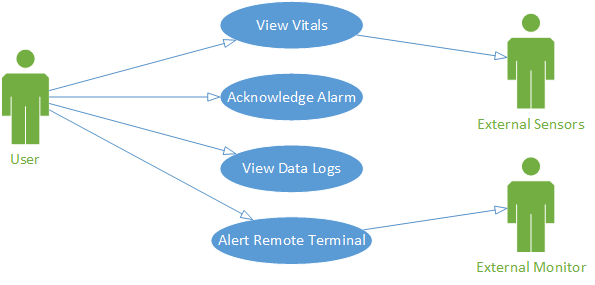
\includegraphics[width=\textwidth]{../design/use_cases_graphical.png}
	\caption{Use case diagram}
	\label{fig:useCases}
\end{figure}

~\\
\textbf{Use Case \#1: View Vital Measurements } \\
In the first use case, the user views the basic measurements picked up by the
sensors connected to the device. \\
During normal operation, once the device is turned on by the user, the system
records the value output by each sensor. This raw value is linearized and 
converted into a human-readable form. Finally, this value is displayed on-screen.

Three exceptional conditions were identified for this use case: 
\begin{itemize}
  \item \emph{One or more of the expected sensors is not connected} - If this occurs, the measurements taken by the device may be erratic. At the present moment, no action will be taken in such events. Later revisions may address the issue
\item \emph{A measured value is outside 5\% of the specified normal range} - In this case, a warning signal will flash as an indication of the warning condition
\item \emph{A measured value falls outside 10\% of a specified "normal" range} - In this case, an audible alarm will sound to indicate the alarm condition
\end{itemize}

~\\
\textbf{Use Case \#2: Acknowledge Alarm} \\
In the second case, the system is in an alarm state. The user acknowledges
the alarm condition by pressing a button.

Upon pressing the button, the system silences the audible alarm. Any visual warnings continue to flash during the silenced period. If a specified amount 
time passes and the sensor reading(s) continue to maintain an alarmed state,
the audible alarm will recommence.

No exceptional conditions were identified for this use case.\\

\subsubsection{Detailed Task Specifications}

\begin{itemize}
  \item
•	Changes to the MeasureTask:
o	Once a complete set of measurements has been taken, the compute task is added to the task queue
o	Pointers to the variables used in the measure task will be relocated to accommodate the new data architecture
o	The pulse measurement will monitor and count the frequency of a pulse rate event interrupt
+	A new value will be stored to memory if the present reading is grater than $\pm$15\% of the previous measurement
+	The measurement limits will correspond to 200bpm and 10bpm, determined empirically. 

•	Changes to ComputeTask:
o	All measurements will be recomputed
o	After computing the corrected values for all measurements, the ComputeTask will remove itself from the task queue

•	Changes to DisplayTask:
o	Display will now support multiple display options
+	Menu mode will allow selection of each of the individual measurements. Upon selection of a measurement, the current value of the measurement will be displayed onscreen
+	Annunciation mode will display the current status of each measurement as in project 1, and provide the same functionality as the display in project 1.

•	Changes to Warn/AlarmTask:
o	The warnings will be activated and indicated as before in project 1
o	The alarm state is changed to activate only when the systolic pressure is 20% above the normal range.
o	The alarm will sound in 1 second tones (1 second on, 1 second off)
o	When an alarm or warning state occurs, the serial communication task will be added to the task queue
o	The deactivation period of the alarm sound is defined as 5 measurement periods

•	New task: Serial Communication:
o	The task is enabled by the warn/alarm task
o	When run, the task will open an RS-232 connection at XXXX baud, XXinsertdetails hereXXX
o	The present corrected measurement will be displayed on the terminal in the same fashion as the display task annunciation mode
o	After sending data to the terminal, the serial communication task will remove itself from the task queue

•	New task: KeypadTask
o	The keypad task will scan the keypad and decode any keypresses
o	The task will have support the following user inputs:
+	Mode selection between 2 modes (1 button)
+	Menu selection between 3 options (1 button)
+	Alarm acknowledgement (1 button)
+	Up and down scroll functionality (1-2 buttons)
o	A new set of global variable will be created to store the state of the keypad and key presses

•	New Task: Initialize (Startup):
o	This task is to run once each time the system is started
o	It will not be part of the task queue
o	It will perform any necessary system initialization, configure and begin the system timebase.
o	After completing these tasks, the task will exit and normal operation will commence.

•	Changes to Schedule:
o	System will maintain a list of activated and deactivated tasks. The list must be updatable during runtime based on the system state
o	The hardware timer will provide a system interrupt every 250ms or equal to the minor cycle, whichever is shorter
o	At runtime, upon a timer interrupt event, all tasks will be added or removed according to the task activation list. The tasks will then be run
o	Task Control Blocks will have forward and backward pointers to allow references to the next task
o	The scheduler cannot block for five seconds
\end{itemize}

\subsection{Software Implementation}

A top-down design approach was used to develop the system.  First, a functional decomposition of the problem was carried out based on the identified use cases.  Next, the system architecture was developed.  After understanding the system architecture, the high-level project file structure in C was defined, followed by the low-level implementation of the tasks.

\subsubsection{Functional Decomposition}

%- User use cases  (need to fix)
%  + Take measurements
%  + Acknowledge alarm
%- High level blocks
%  + Functional decomposition
%    o User
%    o Stellaris board
%    o External Sensors
%  + System Architecture (need to flip inheritance arrows and composition arrow)
%    o Discuss shared data
%    o Discuss TCB->Schedular composition
%    o Discuss TCB->task inheritance
%    o Interaction with hardware
%- Implementation in C
%  + Scheduler
%    o Has queue of TCBs
%    o Runs each with minor cycle delay
%      - Timebase
%        o Specifies major/minor cycle
%  + Tasks
%    o Global data is declared in a header file, globals.h and shared with everyone
%    o Get their own file and header file
%    o Own data is hidden from rest of program, single pointer exposed
%    o Every task gets an initialization to initialize data

After understanding how the user would interact with the device, the system was
functionally decomposed into high-level blocks as shown in
Figure~\ref{fig:func}.  The main system control is located in the CPU, which
controls all data flow into and out of the peripheral devices.  The OLED
displays the user's current vitals including blood pressure (systolic and
diastolic), temperature, and pulse rate.  In the future external sensors will
be added, but for now the values are simulated using the CPU.  The CPU also
controls three LEDs colored green, yellow, and red.  These LEDs are used to
inform the user on the current state of their vitals as well as the state of
the device.  Under normal circumstances, the green LED will be lit.  If the
users' vitals fall outside of a specified range, the red LED will flash at a
specified rate, depending on which vital is out of range.  If the battery is
low, the yellow LED will be illuminated.

\begin{figure}[h]
    \centering
    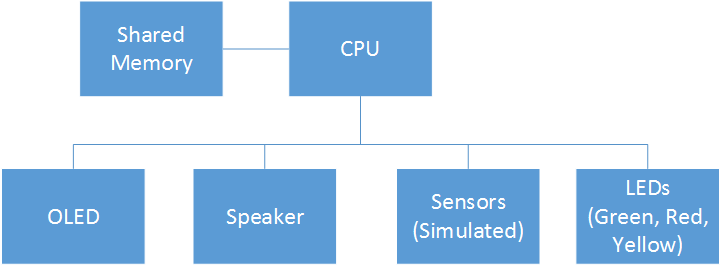
\includegraphics[width=\textwidth]{../design/Functional_decomposition}
    \caption{Functional Decomposition}
    \label{fig:func}
\end{figure}

\subsubsection{System Architecture}
Next, the system architecture was developed (Figure~\ref{fig:arch}).  At a high
level the system works on two main concepts, the scheduler and tasks.  Tasks
embody some sort of work being done, and the scheduler is in charge of
determining the speed and order in which the tasks execute.  The system has
several tasks, each with their own specific job.  For modularity reasons, each
task should have the same public interface and the scheduler should be able to
run each task regardless of that specific tasks job or implementation.  Thus
the task concept is abstracted into a Task Control Block (TCB), and the
scheduler maintains a queue of TCBs to run.  The TCB abstraction is shown in
Figure~\ref{fig:arch} using inheritance, and the fact that the scheduler has a
queue of TCBs is shown with composition.  The core functionality of the system
was divided into the following five main tasks:
\begin{itemize}
  \item \textbf{Measure Task} - In charge of interacting with the blood pressure, temperature, and pulse sensors (simulated)
  \item \textbf{Compute Task} - Converts sensor data into human readable format
  \item \textbf{Display Task} - Displays the measurements on the Stellaris OLED
  \item \textbf{Warning/Alarm Task} - Interacts with the red, yellow, and green LEDs, as well as the speaker to annunciate warning and alarm information
  \item \textbf{Status Task} - Receives battery information from the device
\end{itemize}
Each of these tasks interact using the shared data shown in Figure~\ref{fig:arch}. 

\begin{figure}
    \centering
    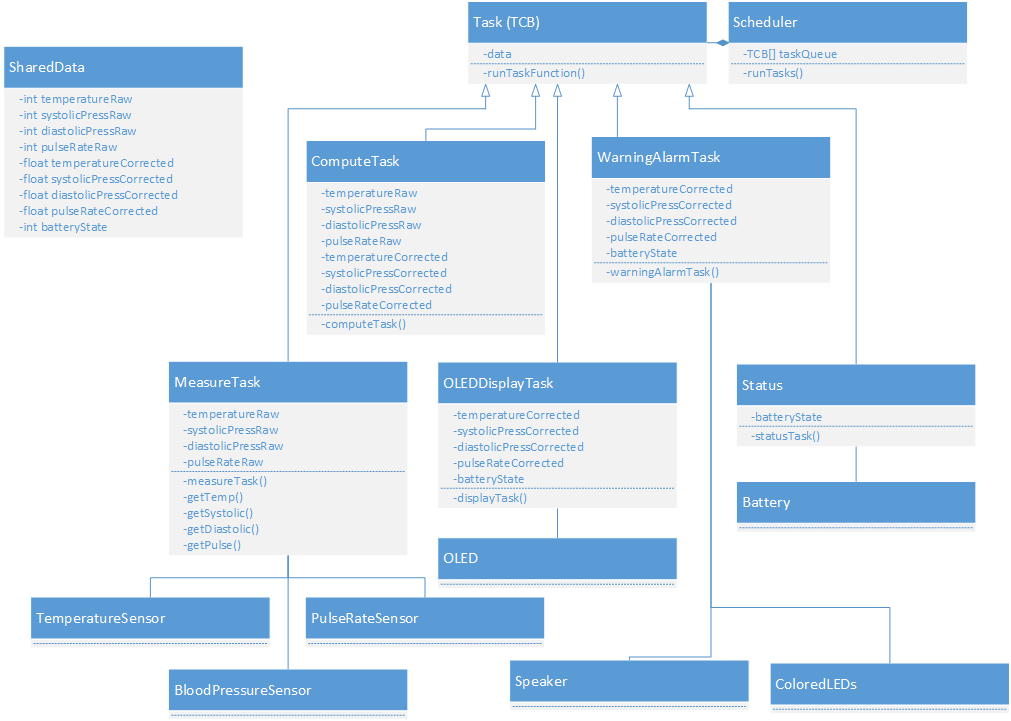
\includegraphics[width=\textwidth]{../design/System_Architecture}
    \caption{System Architecture Diagram}
    \label{fig:arch}
\end{figure}

\subsubsection{High-level Implementation in C}
After developing the system architecture, the design needed to be translated into the C programming language.  The design manifested in a multi-file program consisting of the following source files:
\begin{itemize}
  \item \textbf{globals.c/globals.h} - Used to define the Shared Data used among the tasks
  \item \textbf{schedule.c/schedule.h} - Defines the scheduler interface and it's implementation, as well as the TCB structure
  \item \textbf{timebase.h} - Defines the timebase used for the scheduler and tasks
\end{itemize}
Each task also has it's corresponding ``.c'' and ``.h'' file (for example, measure.c and measure.h).

The TCB structure that the scheduler uses must work for all tasks, and must not
contain any task-specific information.  Instead, the TCB consists of only a void pointer to the tasks data, and a pointer to a function that returns void and takes a void pointer, as follows:
\begin{lstlisting}
struct TCB {
  void *taskDataPtr;
  void (*taskRunFn)(void *);
}
\end{lstlisting}
Leaving out the type information allows the scheduler to pass the task's data
(*taskDataPtr) into the task's run function completely unaware of the kind of
data the task uses or how the task works.

For increased modularity, the data structure used by each task was not put in
the task's header file.  Instead, the structure was declared within the task
implementation file, and instantiated using a task initialization function.  In
the header file, a void pointer pointing to the initialized structure is
exposed with global scope, as well as the task's run and initialization functions.

\subsubsection{Task Implementation}

%implementation details here. Tasks, scheduler, etc. Control diagram goes here,
%activity diagram, etc.
The primary task of this project is to implement C code for a medical device on
the Stellaris EKI-LM3S8962 and its ARM Coretex A3 processor. The project was
started by creating a main file that initializes the variables used in each
task then runs into an infinite while loop. Inside the while loop a run method
is called. The run method is part of the scheduler. This method keeps track of
whether the device is on a minor cycle or a major cycle and runs the preform
task method of each task. The tasks included in this project are Compute,
Measure, Warning, oledDisplay, and status. Each task has a public interface of
2 void pointers. One that when initialized by the main method will point to the
preform task function, and another that, when initialized, points to a struct
containing pointers to the data required by that task. Each task has a task
control block(TCB) in the scheduler. This TCB points contains pointers to the
preform task function and the data for the task. The TCB is used by the
scheduler to run the task. The scheduler contains an array of TCB, each element
in the array corresponds to a new task. In this case there are 5 tasks so 5
elements in the array.The scheduler's run task contains a for loop that runs
through the array of TCB and runs the function pointed to by the TCB with the
argument of the data pointer stored in the TCB. After running all 5 tasks the
TCB has a software defined wait of 250 milliseconds to implement the minor
cycle delay. The software defined wait is simply a for loop that uses addition
as a time consumption tool. It is known that system clock is 8 MHz so having a
for loop go from 0 to 2 million would take about a quarter of a second. The
control flow is shown in Figure~\ref{fig:Control}. 

\begin{figure}[h]
    \centering
    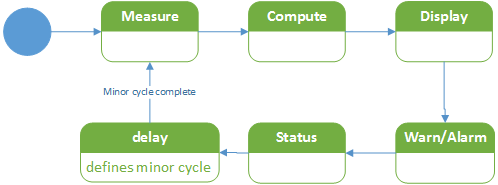
\includegraphics[width=0.8\textwidth]{../design/Control_state_diagram.png}
    \caption{Control Flow Diagram}
    \label{fig:Control}
\end{figure}

Each task has its own unique purpose in the system, and each uses a different
part of the global data. The Measure task (Figure~\ref{fig:measureActivity} in the
appendix), deals only with the raw data from the instruments. This task is
meant to act in place of the instruments that are unavailable. The task only
runs if the scheduler has set the global value is Major Cycle to 1. On a major
cycle the measure function either increments the data of each measurement by 1
or 2 or decrements the data by 1 or 2.

The compute task is very simple. Like the measure task it only runs on a minor
cycle. It takes the raw data that has been set by the measure task, multiplies
by a constant and adds a constant to each piece of raw data to get the
corrected data. The compute task then puts the values for the corrected data in
memory at the location of the global data pointer. Compute uses every data
value except the battery.

After compute, the warning task begins checking for warning or alarm states. The
warning task only deals with the corrected data from compute and the battery
state. This task also must deal with the input and output signals used to
display warning and sound an alarm. Unlike the other tasks, this task has more
to its initialization than just initializing the data. In addition to setting
up the pointers to the global data, during initialization, the task also
enables peripheral banks C, E, F, and G. These are enabled using the
SysCtlPeripheralEnable library call. Additionally the task set up pins C 5, 6,
and 7 as outputs, pins F 0 and G 1 as PWM outputs, and pin E 0 as a pull up
resistor input. Additionally the PWM outputs are set to use a 65 Hz clock to play
a sound at this frequency whenever enabled. The activity diagram is shown in
Figure~\ref{fig:warningActivity} in the appendix. There are 3 subsystems in the
warning task. These subsystems each handle a different part of user
notification. The first subsystem deals with the alarm. The subsystem checks to
see if any of the given corrected data is outside of the range given to us as
acceptable by more than 10\%. If any value is then the PWM output is enabled
using PWMGenEnable. If the values fall back within the acceptable range, or the
user hits the acknowledge button, then the PWM is disabled with PWMGenDisable
and the sound stops. The next subsystem checks the corrected data for being 5\%
out of range of the accepted values. If any value is more than 5\% out of its
range then a warning will be displayed on the red led connected to pin C 5
using the GPIOPinWrite function. Depending on the value that is out of range
the period the led flashes at will vary. The final subsystem is the battery
check. This system checks if there is more than 30\% of battery left on the
device. This is taken from the battery state data field. If there is less than
20\% battery left then a yellow led connected to pin C7 is illuminated, if
there is more then 20\% battery, and the device is not in a warning or alarm
state then the green led on pin C 6 is illuminated. 

To show a user their current medical measurements, the system also has an
oledDisplay task. This task uses the corrected data from measurements, and the
battery state. The display task has an activity diagram shown in
Figure~\ref{fig:displayActivity} in the appendix. This task uses the sprintf()
function in C to convert the data types that the corrected data is stored in,
and properly format these data values into a string which is stored in a
buffer. The string contained in the buffer is then printed to the OLED screen
using the driver library rit128x96x4 functions.

The last task is the status task. This task only deals with one piece of data
which is the battery state data. The only thing the status task does is that on
a major cycle, it decrements the battery state by 1. This is shown in the
activity diagram in Figure~\ref{fig:statusActivity} in the appendix.

\section{Presentation, Discussion, and Analysis of the Results}

\subsection{Results}
The project was completed and demonstrated on January 29, 2014.

Demonstration of the system to the interested parties showed that the system met the requirements initially presented at the onset of the lab project.
Testing of the system prior to demonstration also verified that the system met the specifications listed in Section~\ref{sec:designSpec}.

Additionally, during the demonstration, to show that several warning features worked as expected, source code was temporarily modified to speed up the progression of the system through various warning states. These changes were simple to execute and caused the desired effect on the system without causing unwanted aberrant behavior. Reverting the source code was similarly intuitive.

During the actual coding and implementation of the design, remarks were made several times about the ease of execution during that phase of the project. After the initial high level Design phase, very few changes were made, or required, to the functional design or system architecture.

Using an oscilloscope, the run times of each task were empirically determined. The results are given in Table~\ref{tab:taskRuntimes}.

\begin{table}[h]
	\centering
	\begin{tabular}{|l|r|} 
		\hline
		Task & Runtime ($\mu$s) \\ \hline
		Measure & 23.4 \\ \hline
		Compute & 55.4 \\ \hline
		Display & 22900.0 \\ \hline
		Warning & 27.4	\\ \hline
		Status & 5.6	\\ \hline
	\end{tabular}
	\caption{Empirically determined task runtimes}
  \label{tab:taskRuntimes}
\end{table}

\textbf{Answers to the last three questions in the list of items to include in the project report:}
\emph{You don't find the stealth submarine. That's why they are so expensive; at that cost, you take great pains to never lose one.\\
A helium balloon always rises. It just rises upside-down. \\
If you really managed to lose the stealth submersible, you first have to tell the government, which will deny it has any stealth submersibles, then you have to comb the seven seas until your comb hits the sub.}
 
\subsection{Discussion of Results}
The ease of change in the code is the result of a large amount of time spent on
design.  The design makes it easy to configure flash times, add new tasks, and
to reason about tasks independently of the whole system.  The solid high-level
architectural design led to ease of implementation and change.

In terms of performance, the run times of each task appear to correspond with
the number of instructions required for each task.  Given the speed of the CPU,
8 MHz, we can calculate an estimated number of instructions for each task.
This is given in Table~\ref{tab:instr}.
\begin{table}[h]
	\centering
	\begin{tabular}{|l|r|} 
		\hline
		Task & Instructions \\ \hline
		Measure & 187 \\ \hline
		Compute & 443 \\ \hline
		Display & 183,200 \\ \hline
		Warning & 219	\\ \hline
		Status & 45	\\ \hline
	\end{tabular}
	\caption{Estimated instructions per task, rounded to the nearest instruction}
  \label{tab:instr}
\end{table}
The majority of the cycles are likely spent waiting for memory.  For example,
the status task only has two comparisons and an arithmetic operation, but has
to reference the data in global memory.  The exception here is the display
task, which was about three orders of magnitude more instructions than the
other tasks.  This was due to the sprintf() library call, included in the
standard C library.  While this could have been optimized, it was found that
with a minor cycle delay of 250 ms, the display delay of 22.9 ms was not
significant.


\subsection{Analysis of Any Errors}
The project was completed without any residual errors or unsolved problems. See the following section for analysis of issues encountered while working on the project itself.

\subsection{Analysis of Implementation Issues and Workarounds}

%State any problems you encountered while working on the project. If your project did not work or worked only partially, provide an analysis of why and what efforts were made to identify the root cause of any problems. \\

%Some points to bring up: did not enable the GPIO bank (caused OLED display to not work), could not get switch to work (solved by understanding that switch required pull up). P or J can talk about design solutions that did not work. On the whole,  had problems with going too deep, too quickly.

The medical instrument design in this project was completed and tested successfully to meet all the requirements, the designers did face a number of errors and difficulties in the process. Most of the challenges faced in this design were in implementing the inputs and outputs from the ARM micro processor. In this implementation, the students originally consulted the driver library documentation and found how to enable a general purpose input output (GPIO) pin, and how to read from a GPIO pin. However, when the code to enable a GPIO pin was executed, the execution of tasks within the scheduler froze completely until a reset. This problem was caused by the students failure to enable the peripheral bank that the GPIO pins existed on. After learning how to do this, code was added to enable the peripheral and the task execution no longer froze on enabling a pin.

Another problem encountered by the design team was that initially after setting up a GPIO pin as an input to take a button press from the Stellaris test board, pressing the button did not have the intended effect. The push button did not change the state of the input. The students were originally perplexed and tried a number of solutions to this problem. Testing indicated that the code for the GPIO input was correct as a 3.3 V signal directly to the pin could trigger the intended event on the input. Eventually it was found that to use the push button switch the GPIO pin's pad must be configured to accept a pull up resistor type of input.

All problems were solved before demonstrating the product to the interested parties. As such, the final design did not have any errors.

\section{Test Plan}

To ensure that this project meets the specifications listed in 
section~\ref{sec:designSpec}, the following parts of the system must be 
tested: 

\begin{itemize}
	\item Vitals are measured and updated
	\item System properly displays corrected measurements and units properly
	\item System enters, indicates, and exits the proper warning state for blood pressure, temperature, pulse, and battery
	\item System enters and exits the alarm state correctly
	\item Alarm is silenced upon button push
	\item Alarm recommences sound after silencing if system remains in alarm state longer than silence period
\end{itemize}

Additional tests to determine the runtime of each specific task are also required.

\subsection{Test Specification}

Annotated description of what is to be tested and the test limits.  This specification quantifies inputs, outputs, and constraints on the system.  That is, it provides specific values for each. 

Note, this does not specify test implementation...this is what to do, not how to do it.

\subsubsection{Scheduler}
The scheduler needs to be shown to correctly schedule and dispatch tasks.  This means that task should execute in the right order, and at the right time.  Given a minor cycle of 50 ms, every task should run roughly once every 50 ms.  

\subsubsection{Measure Task}
For this design, no external sensors were used; instead they were simulated.  Each simulated sensor should be tested and verified against the specification, as follow.
\begin{itemize}
  \item \textbf{Temperature} The temperature should increase by two every even major cycle (5 seconds) and decrease by one ever odd major cycle until it exceeds 50, at which point the process should reverse (decrease by two every even major cycle and increase by one every odd major cycle), until it dips below 15, and the whole process should be started over again.  
  \item \textbf{Pulse} The pulse requirements are very similar to measure, except the pulse should increase by three rather than two, and the range is between 15 and 40.
  \item \textbf{Systolic Pressure} The systolic pressure should increase by three every even major cycle and decreases by one every odd major cycle.  If it exceeds 100, it should reset to an initial value.
  \item \textbf{Diastolic Pressure} The diastolic pressure should decrease by two on even major cycles and decrease by one on odd major cycles, until it drops below 40, when it should restart the process.
\end{itemize}

\subsubsection{Compute Task}
The compute task should be verified to convert raw simulated sensor data according to the following formulas.
\begin{itemize}
  \item $CorrectedTemperature = 5 + 0.75 * RawTemperature$
  \item $CorrectedSystolicPressure = 9 + 2 * RawSystolicPressure$
  \item $CorrectedDiastolicPressure = 6 + 1.5 * RawTemperature$
  \item $CorrectedPulseRate = 8 + 3 * RawTemperature$
\end{itemize}

\subsubsection{Display Task}
The display task should be tested to print each corrected value properly on the screen, and update them as the computations are done.

\subsubsection{Warning/Alarm Task} 
The warning/alarm system needs to be tested to do several things.  When in a
warning state, it should flash the red LED at the rate appropriate for the
warning.  When the battery is low, it should illuminate the yellow LED.  If the
system is in an alarm state, it should sound the speaker alarm.  The following
ranges in Table~\ref{tab:ranges} are calculated from the specified minimum and
maximums found in Table~\ref{tab:sensorDefs} on page \pageref{tab:sensorDefs}.
\begin{table}[h]
	\centering
	\begin{tabular}{lcr} 
    \toprule
		Data & Warning Range & Alarm Range \\
		\midrule
		Temperature & 34.3 - 39.7 C & 32.5 - 41.6 C\\
		Systolic Pressure  & $>$ 84 mmHg & $>$ 88 mmHg\\
		Diastolic Pressure & $>$ 126 mmHg & $>$ 132 mmHg\\
		Pulse & 57 - 63 BPM & 54 - 110 BPM \\
    \bottomrule
	\end{tabular}
	\caption{Initial values and warning/alarm states}
  \label{tab:ranges}
\end{table}

\subsubsection{Status Task}
Since the initial design does not use a battery, the status task simulates the
battery state using the CPU.  For now, it simply decrements the state of the
battery.  The test should show that the battery state is decremented by one
every major cycle.

\subsection{Test Cases}

The students begin testing by examining if the alarm sounds at the proper time.
This is initially tested by disabling the functions that simulate measurements
being made on each of the data measurements, and setting their initial values
to be either within the alarm range or outside of the alarm range. The warning
states were also initially tested this way. The initial values for raw data
given in Table~\ref{tab:sensorDefs} on page \pageref{tab:sensorDefs} were used
to test the normal state of the machine because each falls within the
acceptable range of measurements for corrected data (also given in
Table~\ref{tab:sensorDefs}) that does not require a warning.
	
Using these initial values, the code was programmed onto the Stellaris board.
Correct operation was verified by the alarm not sounding, and the red led being
off, indicating that no warning state was in effect. In addition the green led
was on indicating a normal state. Next the students varied one parameter at a
time to be outside of the acceptable range by more than 10\%. Starting with the
temperature being set to an initial raw value of 50, the alarm was verified by
hearing the aural annunciation coming from the system. In addition, the
temperature warning stat was also in effect. This means that the green led was
off and the red led was blinking. To verify correct operation we needed to make
sure the led was blinking with a period of 1 second. The correct flashing
pattern was verified by counting the number of times the led flashed in 6
seconds. In this case, for temperature, the led flashed 6 times in 6 seconds
indicating a 1 second period, and correct operation. After this test, the
temperature value was returned to 42 and the Pulse was instead set to 45. The
same methods were used to verify that the alarm and warning states for pulse
rate were working correctly, but this time the warning led turned on 3 times in
6 seconds indicating a 2 second period which is the intended period of
flashing. The pulse rate was then returned to 25 and each pressure reading was
checked for correct operation individually by being set to an initial raw value
of 100. Once again, the green led started off because the system was not in a
normal state. The alarm was sounding due to the extremely high blood pressure
measurements, and the red warning led flashed 12 times in 6 seconds indicating
the correct period of .5 seconds for a blood pressure warning. In addition to
testing the validity of each warning state and alarm state, the acknowledgement
of the alarm was also tested during each of these tests. This was tested by
hitting the acknowledge button once during each measurements test. During each
test, hitting the acknowledge button turned the alarm sound off for a short
time, as intended. 

Next the measurement simulation functions were tested. This was done by
re-enabling each one that had been disabled from the previous test one at a
time. The initial raw values were again set to the values in Figure 5. When
each measurement was re-enabled, the students could watch the temperature change
at each major cycle using the OLED display. Since the OLED display indicated
that the corrected temperature went up .75 degrees on a major cycle then down
1.5 degrees on the next, the temperature measurement was working as intended.
This situation also gave the students an opportunity to verify that the warning
and alarm states initiated as the temperature fell out of the acceptable range.
The Led began flashing with a 1 second period after a few major cycles, then
the alarm began sounding, indicating correct operation. Since temperature was
working correctly, the temperature measurement function was once again disabled
and the pulse rate measurement function was re-enabled. The OLED display
indicated that the pulse rate was increasing by 3 on a major cycle then falling
by 6 on the following major cycle. This was consistent with the intended
design. The alarm and warning being initiated as the pulse rate fell. The pulse
rate measurement was then disabled and each blood pressure measurement was
re-enabled individually for testing. The Systolic pressure began by rising 4 mm
Hg on a major cycle then falling 2 mm Hg on the next, and the Diastolic
pressure by rising 3 on a Major cycle and falling 1.5 on the next, this was
consistent with our design. The warning and alarm states were activated as each
passed its threshold and the red led was blinking with a period of .5 seconds.
The warning led was also tested in the case that all warning states were
active. To do this all initial values were set to 100. In this case, as
designed by the students, the red warning led indicated the fastest blinking
warning with a .5 second period. 

The final bit of testing preformed on the system was timing each task within
the system. This was done by adding a general purpose output pin in our
scheduler code. This output was set high right before the execution of a task,
and set low immediately after the execution of the task. An oscilloscope was
then attached to this output pin and set to trigger on a positive edge. The
cursors were then used to measure the amount of time the signal was high in
each cycle.
	
Using these initial values, the code was programmed onto the Stellaris board.
Correct operation was verified by the alarm not sounding, and the red led being
off, indicating that no warning state was in effect. In addition the green led
was on indicating a normal state. Next the students varied one parameter at a
time to be outside of the acceptable range by more than 10\%. Starting with the
temperature being set to an initial raw value of 50, the alarm was verified by
hearing the aural annunciation coming from the system. In addition, the
temperature warning stat was also in effect. This means that the green led was
off and the red led was blinking. To verify correct operation the students
needed to make sure the led was blinking with a period of 1 second. The correct
flashing pattern was verified by counting the number of times the led flashed
in 6 seconds. In this case, for temperature, the led flashed 6 times in 6
seconds indicating a 1 second period, and correct operation. After this test,
the temperature value was returned to 42 and the Pulse was instead set to 45.
The same methods were used to verify that the alarm and warning states for
pulse rate were working correctly, but this time the warning led turned on 3
times in 6 seconds indicating a 2 second period which is the intended period of
flashing. The pulse rate was then returned to 25 and each pressure reading was
checked for correct operation individually by being set to an initial raw value
of 100. Once again, the green led started off because the system was not in a
normal state. The alarm was sounding due to the extremely high blood pressure
measurements, and the red warning led flashed 12 times in 6 seconds indicating
the correct period of .5 seconds for a blood pressure warning. In addition to
testing the validity of each warning state and alarm state, the acknowledgement
of the alarm was also tested during each of these tests. This was tested by
hitting the acknowledge button once during each measurements test. During each
test, hitting the acknowledge button turned the alarm sound off for a short
time, as intended. 

Next the measurement simulation functions were tested. This was done by
re-enabling each one that had been disabled from the previous test one at a
time. The initial raw values were again set to the values in Figure 5. When
each measurement was re-enabled, the students could watch the temperature change
at each major cycle using the OLED display. Since the OLED display indicated
that the corrected temperature went up .75 degrees on a major cycle then down
1.5 degrees on the next, the temperature measurement was working as intended.
This situation also gave the students an opportunity to verify that the warning
and alarm states initiated as the temperature fell out of the acceptable range.
The Led began flashing with a 1 second period after a few major cycles, then
the alarm began sounding, indicating correct operation. Since temperature was
working correctly, the temperature measurement function was once again disabled
and the pulse rate measurement function was re-enabled. The OLED display
indicated that the pulse rate was increasing by 3 on a major cycle then falling
by 6 on the following major cycle. This was consistent with the intended
design. The alarm and warning being initiated as the pulse rate fell. The pulse
rate measurement was then disabled and each blood pressure measurement was
re-enabled individually for testing. The Systolic pressure began by rising 4 mm
Hg on a major cycle then falling 2 mm Hg on the next, and the Diastolic
pressure by rising 3 on a Major cycle and falling 1.5 on the next, this was
consistent with the design. The warning and alarm states were activated as each
passed its threshold and the red led was blinking with a period of .5 seconds.
The warning led was also tested in the case that all warning states were
active. To do this all initial values were set to 100. In this case, as
designed by the students, the red warning led indicated the fastest blinking
warning with a .5 second period. 

The final bit of testing preformed on the system was timing each task within
the system. This was done by adding a general purpose output pin in the
scheduler code. This output was set high right before the execution of a task,
and set low immediately after the execution of the task. An oscilloscope was
then attached to this output pin and set to trigger on a positive edge. The
cursors were then used to measure the amount of time the signal was high in
each cycle.

\section{Summary and Conclusion}

\subsection{Final Summary} The students began creating their medical instrument
through a rigorous design process at different levels of detail. The students
then continued work by implementing their design in C code for the ARM Cortex
A3 microprocessor. Next the code was tested and debugged using the IAR
workbench debugging tool, as well as visual queues programmed into the design.
Finally, after verifying that the system worked as specified, it was presented
to the instructor.

\subsection{Project Conclusions} This project contained 3 major phases, the
design, implementation, and testing steps. The students were immediately
introduced to using the unified modeling language(UML) to design embedded
systems. This is the first time many students will have used UML for system
design which caused some confusion and difficulty. In the end through the use
of the UML guidelines for design, the students were able to implement their
system in code for the Texas Instruments Stellaris EKI-LM3S8962 much more
quickly and with far fewer errors than if they had spent less time in the
design phase of this project. 

Effective design tools allowed the students to quickly implement their embedded system in C code for an ARM Cortex A3 processor, and move onto the testing phase of the project quickly. Unfortunately, while testing the students encountered a number of problems in using the PWM and general purpose input and output signals. After consulting the documentation for the Stellaris kit and solving their input/output problems, they began testing their design using visual and audio queues, the IAR embedded workbench debugger, and a few specifically programmed debug features. After the results of the testing verified the design to be working correctly, the students proceeded to present their medical instrument to their instructor.

\pagebreak
\appendix

\section{Breakdown of Lab Person-hours (Estimated)}

\begin{tabular}{|l|*{4}{r|}}
	\hline
	Person & Design Hrs & Code Hrs & Test/Debug Hrs & Documentation Hrs \\ \hline
	Patrick & 15 & 7 & 2 & 9  \\ \hline
	Jarret & 3 & 6 & 6 & 7  \\ \hline
	Jonathan & 15 & 5 & 4 & 8  \\ \hline
\end{tabular}

~\\

By initializing/signing above, I attest that I did in fact work the estimated number of hours stated. I also attest, under penalty of shame, that the work produced during the lab and contained herein is actually my own (as far as I know to be true). If special considerations or dispensations are due others or myself, I have indicated them below.

\pagebreak

\section{Activity Diagrams}

\begin{figure}
  \centering
  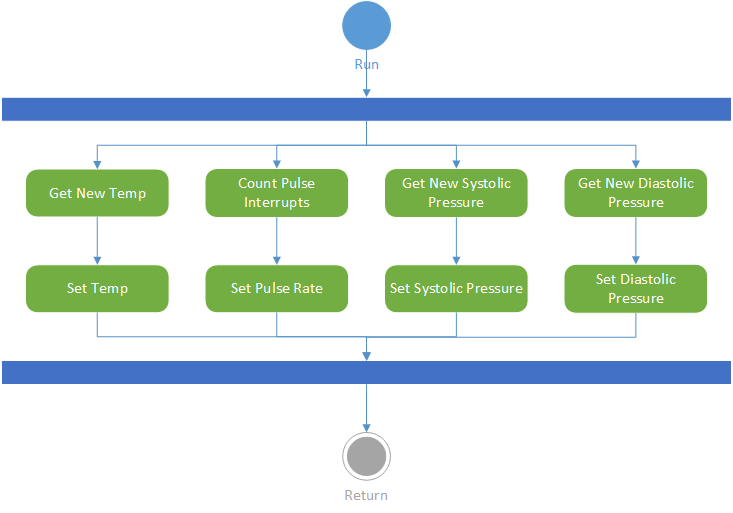
\includegraphics[width=\textwidth]{../design/measure_activity.png}
  \caption{Measure Activity Diagram}
  \label{fig:measureActivity}
\end{figure}

\begin{figure}
  \centering
  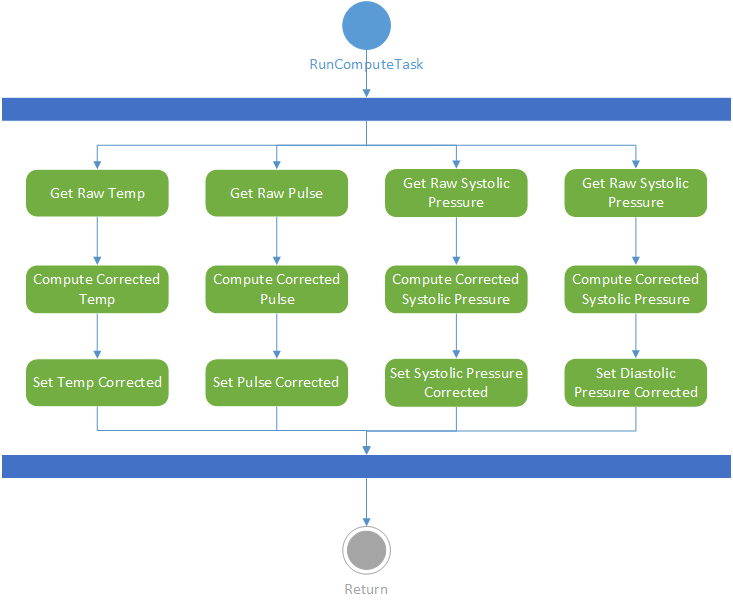
\includegraphics[width=\textwidth]{../design/compute_activity.png}
  \caption{Compute Activity Diagram}
  \label{fig:computeActivity}
\end{figure}

\begin{figure}
  \centering
  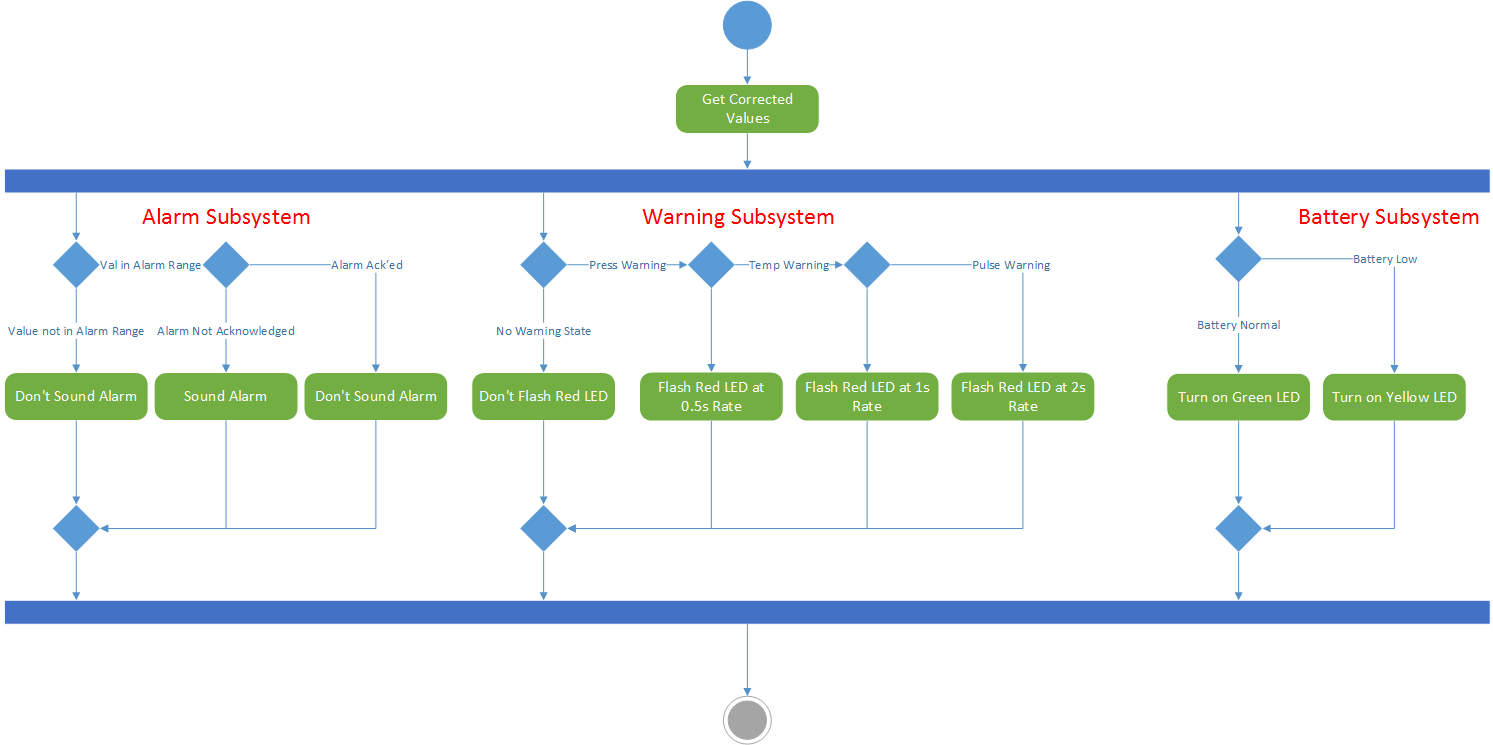
\includegraphics[width=\textwidth]{../design/warning_activity.png}
  \caption{Warning Activity Diagram}
  \label{fig:warningActivity}
\end{figure}

\begin{figure}
  \centering
  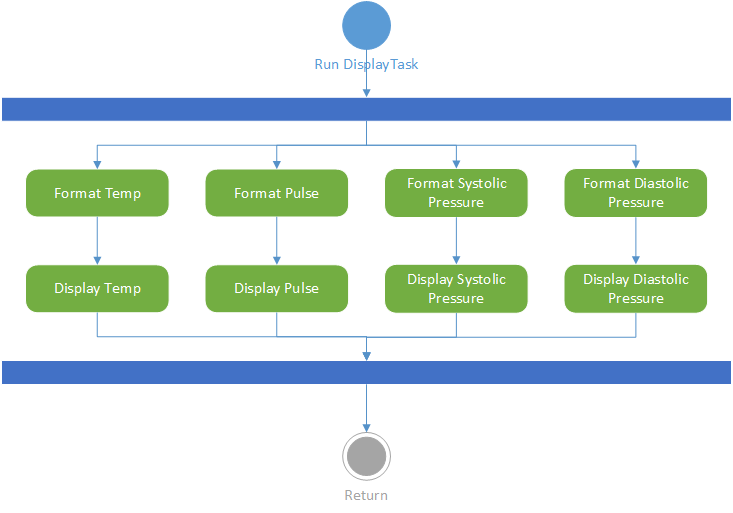
\includegraphics[width=\textwidth]{../design/display_activity.png}
  \caption{Display Activity Diagram}
  \label{fig:displayActivity}
\end{figure}

\begin{figure}
  \centering
  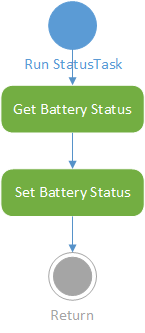
\includegraphics[width=0.2\textwidth]{../design/Status_activity.png}
  \caption{Status Activity Diagram}
  \label{fig:statusActivity}
\end{figure}

\pagebreak

\section{Source Code}

Source code for this project is provided below.

\subsection{Main Function}
\lstinputlisting{../code/main.c}

\subsection{Global Data}
\lstinputlisting{../code/globals.h}
\lstinputlisting{../code/globals.c}

\subsection{Timebase}
\lstinputlisting{../code/timebase.h}

\subsection{Scheduler}
\lstinputlisting{../code/schedule.h}
\lstinputlisting{../code/schedule.c}

\subsection{Tasks}
\subsubsection{Measure Task}
\lstinputlisting{../code/measure.h}
\lstinputlisting{../code/measure.c}

\subsubsection{Compute Task}
\lstinputlisting{../code/compute.h}
\lstinputlisting{../code/compute.c}

\subsubsection{Display Task}
\lstinputlisting{../code/display.h}
\lstinputlisting{../code/display.c}

\subsubsection{Warning/Alarm Task}
\lstinputlisting{../code/warning.h}
\lstinputlisting{../code/warning.c}

\subsubsection{Status}
\lstinputlisting{../code/status.h}
\lstinputlisting{../code/status.c}

\end{document}
